\documentclass{article}
\usepackage[utf8]{inputenc}
\usepackage{amsmath}
\usepackage[english, russian]{babel}
\usepackage{euscript}
\usepackage{mathrsfs}
\usepackage{amssymb}
\usepackage{graphicx}
\usepackage[12pt]{extsizes}
\renewcommand{\familydefault}{\rmdefault}
\title{\textbf {Идеи решения задач тысячелетия путем дифференцированного исчисления}}
\author{Мишенков Даниил Николаевич,\\
		доцент кафедры высшей философии МГУ}
\date{\textit {\normalsize {ноябрь 2022}}}
\begin{document}
\maketitle
\section {}
Рассмотрим следующую функцию:\newline
\[f(x) = \sin( x^{ 3 })+(\cos( x))^{ 2 }\]\newline
Очевидно, что понять логику ее работы просто так невозможно, поэтому необходимо провести комплексный анализ данной функции.\newline\newline
Упростим функцию, чтобы с ней было более удобно работать.\newline
Получим следующий результат:\newline\newline
\[f(x) = \sin( x^{ 3 })+(\cos( x))^{ 2 }\]\newline
Найдем значение функции в точке 0.00 знаменитым в 17 веке методом буль-буль\newline
\[f(a) = 1.00, где a = 0.00\]\newline
Найдем производную 2 порядка этой функции методом Шварцвальда III\newline
Очевидно, что\newline
\[( x)' =  1 \]\newline
Читатель, в качестве упражнения, может проверить, что\newline
\[(\cos( x))' = \sin( x)\cdot -1 \cdot 1 \]\newline
Более содержительным является следующий результат\newline
\[((\cos( x))^{ 2 })' = \cos( x)\cdot\sin( x)\cdot -1 \cdot 2 \]\newline
Очевидно, что\newline
\[( x)' =  1 \]\newline
Читатель, в качестве упражнения, может проверить, что\newline
\[( x^{ 3 })' =  x^{ 2 }\cdot 3 \]\newline
Более содержительным является следующий результат\newline
\[(\sin( x^{ 3 }))' = \cos( x^{ 3 })\cdot x^{ 2 }\cdot 3 \]\newline
А тут так\newline
\[(\sin( x^{ 3 })+(\cos( x))^{ 2 })' = \cos( x^{ 3 })\cdot x^{ 2 }\cdot 3 +\cos( x)\cdot\sin( x)\cdot -1 \cdot 2 \]\newline
Очевидно, что\newline
\[( 2 )' =  0 \]\newline
Очевидно, что\newline
\[( -1 )' =  0 \]\newline
Очевидно, что\newline
\[( x)' =  1 \]\newline
Читатель, в качестве упражнения, может проверить, что\newline
\[(\sin( x))' = \cos( x)\cdot 1 \]\newline
Более содержительным является следующий результат\newline
\[(\sin( x)\cdot -1 )' = \cos( x)\cdot -1 + 0 \]\newline
Очевидно, что\newline
\[( x)' =  1 \]\newline
Читатель, в качестве упражнения, может проверить, что\newline
\[(\cos( x))' = \sin( x)\cdot -1 \cdot 1 \]\newline
Более содержительным является следующий результат\newline
\[(\cos( x)\cdot\sin( x)\cdot -1 )' = \sin( x)\cdot -1 \cdot\sin( x)\cdot -1 +\cos( x)\cdot\cos( x)\cdot -1 \]\newline
А тут так\newline
\[(\cos( x)\cdot\sin( x)\cdot -1 \cdot 2 )' =  A_{1} + 0 \]\newline
где:\[A_{1} = (\sin( x)\cdot -1 \cdot\sin( x)\cdot -1 +\cos( x)\cdot\cos( x)\cdot -1 )\cdot 2 \]
А тут так\newline
\[( 3 )' =  0 \]\newline
А тут так\newline
\[( x)' =  1 \]\newline
Получен важнейший результат\newline
\[( x^{ 2 })' =  x\cdot 2 \]\newline
Более содержительным является следующий результат\newline
\[( x^{ 2 }\cdot 3 )' =  x\cdot 2 \cdot 3 + 0 \]\newline
А тут так\newline
\[( x)' =  1 \]\newline
Получен важнейший результат\newline
\[( x^{ 3 })' =  x^{ 2 }\cdot 3 \]\newline
Более содержительным является следующий результат\newline
\[(\cos( x^{ 3 }))' = \sin( x^{ 3 })\cdot -1 \cdot x^{ 2 }\cdot 3 \]\newline
В СССР следующий результат было стыдно записывать\newline
\[(\cos( x^{ 3 })\cdot x^{ 2 }\cdot 3 )' =  A_{2} +\cos( x ^{ 3 })\cdot x \cdot 2 \cdot 3 \]\newline
где:\[A_{2} = \sin( x^{ 3 })\cdot -1 \cdot x^{ 2 }\cdot 3 \cdot x^{ 2 }\cdot 3 \]
В СССР следующий результат было стыдно записывать\newline
\[(\cos( x^{ 3 })\cdot x^{ 2 }\cdot 3 +\cos( x)\cdot\sin( x)\cdot -1 \cdot 2 )' =  A_{3} + A_{4} \]\newline
где:\[A_{3} = \sin( x^{ 3 })\cdot -1 \cdot x^{ 2 }\cdot 3 \cdot x^{ 2 }\cdot 3 +\cos( x^{ 3 })\cdot x\cdot 2 \cdot 3 \]
\[A_{4} = (\sin( x)\cdot -1 \cdot\sin( x)\cdot -1 +\cos( x)\cdot\cos( x)\cdot -1 )\cdot 2 \]
Для простоты запишем этот результат так:\newline
\[f^{(2)}(x) = \sin( x^{ 3 })\cdot -1 \cdot x^{ 2 }\cdot 3 \cdot x^{ 2 }\cdot 3 +\cos( x^{ 3 })\cdot x\cdot 2 \cdot 3 +(\sin( x)\cdot -1 \cdot\sin( x)\cdot -1 +\cos( x)\cdot\cos( x)\cdot -1 )\cdot 2  A_{5} + A_{6} \]\newline
где:\[A_{5} = \sin( x^{ 3 })\cdot -1 \cdot x^{ 2 }\cdot 3 \cdot x^{ 2 }\cdot 3 +\cos( x^{ 3 })\cdot x\cdot 2 \cdot 3 \]
\[A_{6} = (\sin( x)\cdot -1 \cdot\sin( x)\cdot -1 +\cos( x)\cdot\cos( x)\cdot -1 )\cdot 2 \]
Разложим функцию (по Тейлору) до $o(x^{2})$ в точке a = 0.00\newline
\[f(a) =  1 + -1 \cdot x^{ 2 }\]\newline
Найдем касательную в точке a = 1.00:
\[t(x) =  1.13 + 0.71 \cdot( x- 1 )\]\newpage
\begin{figure}[h]
\centering
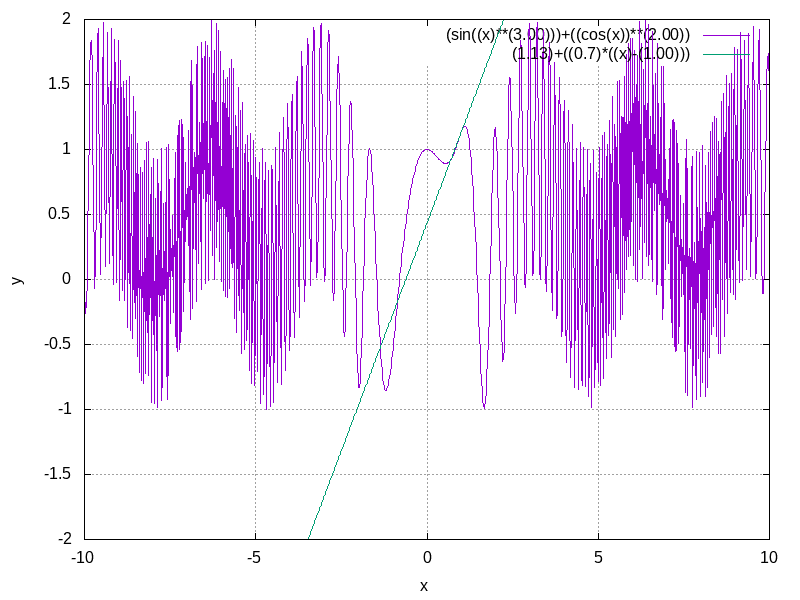
\includegraphics[width=0.8\linewidth]{func.png}
\caption{график функций полученный после комплексного анализа}
\label{fig:mpr}
\end{figure}
\end {document}